\documentclass[8pt]{article}
\usepackage{amsmath}
\usepackage{amssymb}
\usepackage[
    left=0.5in,
    right=0.5in,
    top=0.5in,
    bottom=0.5in
]{geometry}
\usepackage{graphicx}
\usepackage{color}
\usepackage{multicol} % Added for two columns
\usepackage{tabularx} % For better tables
\usepackage{array}    % For column formatting

\setlength{\parindent}{0pt}
% \setlength{\parskip}{0pt}
\def\chpiv@path{../../../Chp 4}

\begin{document}

\begin{center}
    {\LARGE \textbf{MA213 Quiz 4 Formula Sheet}}
\end{center}

\vspace{1em}

\input{../fsheet_pg1}

% R Functions Table, tdist_picture.png and pnorm_picture.png side by side
\begin{center}
\begin{minipage}[t]{0.40\textwidth}
\vspace{0pt} % Align tops
\begingroup
\setlength{\tabcolsep}{4pt} % reduce horizontal padding
\renewcommand{\arraystretch}{1.3}
\scriptsize % smaller font to "squish" the table
\begin{tabularx}{\textwidth}{|>{\raggedright\arraybackslash}p{0.28\linewidth}|>{\raggedright\arraybackslash}X|}
\hline
\textbf{Distribution} & \textbf{R Functions} \\
\hline
Normal & \texttt{rnorm}, \texttt{dnorm}, \texttt{pnorm}, \texttt{qnorm} \\
\hline
Geometric & \texttt{rgeom}, \texttt{dgeom}, \texttt{pgeom}, \texttt{qgeom} \\
\hline
Binomial & \texttt{rbinom}, \texttt{dbinom}, \texttt{pbinom}, \texttt{qbinom} \\
\hline
Poisson & \texttt{rpois}, \texttt{dpois}, \texttt{ppois}, \texttt{qpois} \\
\hline
\end{tabularx}

\vspace{0.4em}
\textbf{r} -- generate random number; \textbf{d} -- PDF or PMF; \textbf{p} -- CDF;\\ \textbf{q} -- inverse CDF
\endgroup
\end{minipage}%
\hfill
\begin{minipage}[t]{0.55\textwidth}
\vspace{0pt} % Align tops
\centering
% two small pictures side-by-side (pnorm and tdist) scaled to fit the narrow column
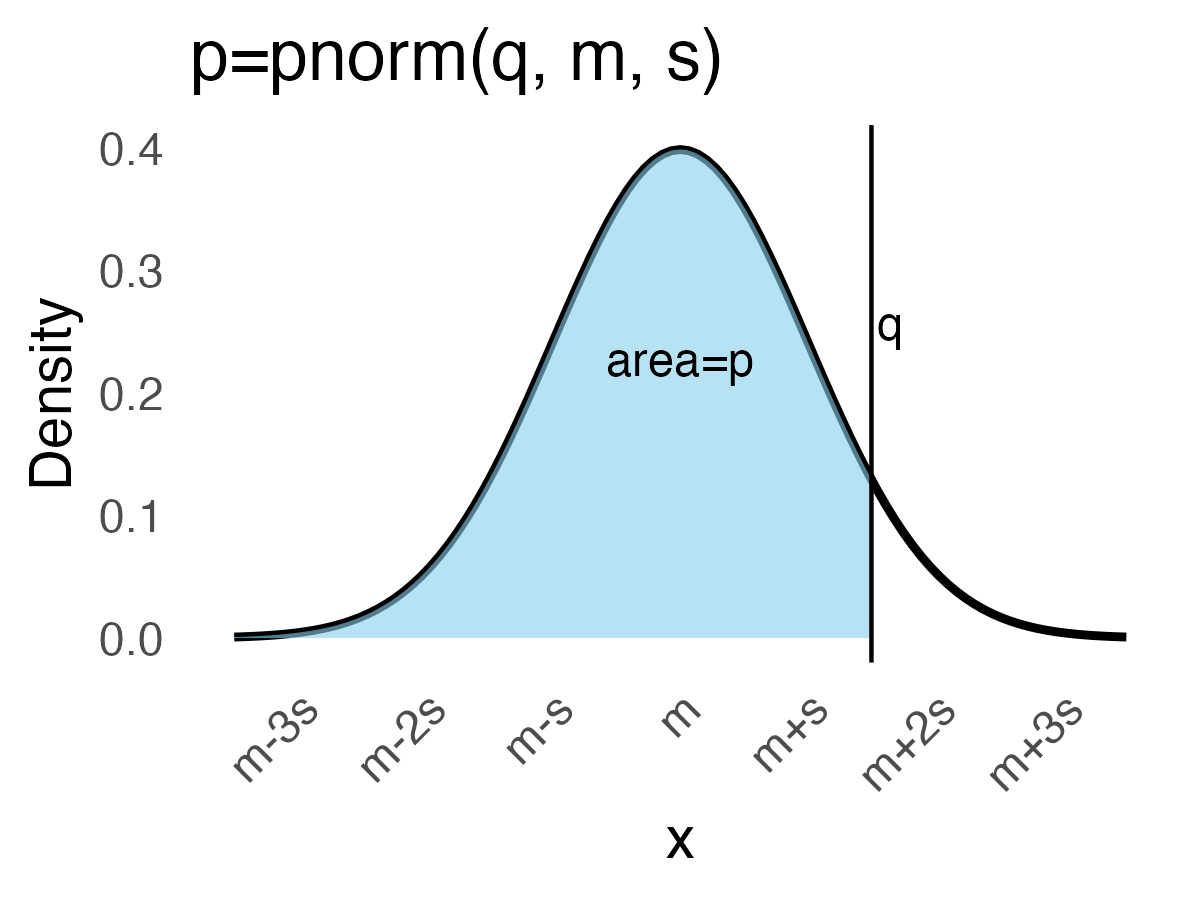
\includegraphics[width=0.48\linewidth]{../figures/pnorm_picture}\hfill
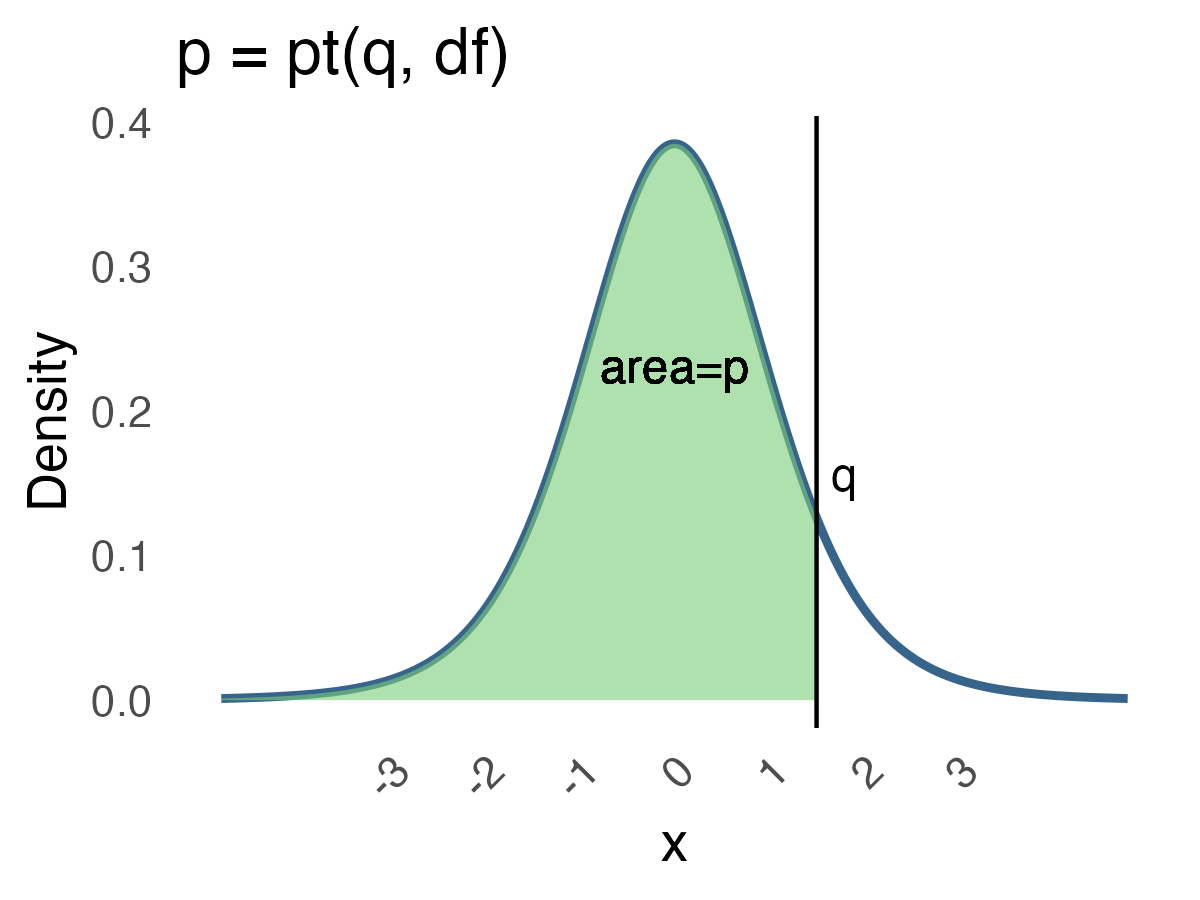
\includegraphics[width=0.48\linewidth]{../figures/tdist_picture}
\end{minipage}
\end{center}

\clearpage

\begin{multicols}{2} % Begin two columns

\textbf{Common Point Estimates and their Sampling Distributions}

\textit{Single Proportion:}
\begin{align*}
    &\hat{p} = \frac{X}{n} \quad \text{(Sample proportion)} \\
    &Pr\left(\hat{p}=\frac{k}{n}\right) = \binom{n}{k} p^k (1-p)^{n-k} \\
    &\hat{p} \stackrel{\text{approx}}{\sim} \text{Normal}\left(p, \sqrt{\frac{p(1-p)}{n}}\right) \\
\end{align*}
\textit{Difference of Two Proportions (independent samples):}
\begin{align*}
    &\hat{p}_1 - \hat{p}_2 \quad \text{(Independent)} \\
    &(\hat{p}_1 - \hat{p}_2) \stackrel{\text{approx}}{\sim} \text{Normal}\left(p_1 - p_2, \sqrt{\frac{p_1(1-p_1)}{n_1} + \frac{p_2(1-p_2)}{n_2}}\right)
\end{align*}
\textit{Conditions for normality (Proportions):}
\begin{itemize} 
    \item Independence: Random sample/independent observations; 10\% condition: $n \leq 0.1N$
    \item Normality: Success-failure condition: $np \ge 10$ and $n(1-p) \ge 10$
\end{itemize}



\textit{Single Mean: (known $\sigma$)}
\[\bar{X} = \frac{1}{n} \sum_{i=1}^{n} X_i \qquad \bar{X} \stackrel{\text{approx}}{\sim} \text{Normal}\left(\mu, \frac{\sigma}{\sqrt{n}}\right)\]
\textit{Conditions for normality (Means):}
\begin{itemize} 
    \item Independence: Random sample/independent observations; 10\% condition: $n \leq 0.1N$
    \item Normality: Exact when the population distribution is Normal; Approximate when $n>30$
\end{itemize}
\textit{Single Mean: (unknown $\sigma$)}
\[
    \frac{\bar{X}-\mu}{s/\sqrt{n}} \sim t_{df} \qquad
    df = n - 1
\]
\textit{Difference of Two Means (paired samples):}
\begin{itemize}
    \item Same as single mean, but on the differences \[D_i = X_{1i} - X_{2i}\]
\end{itemize}
% \columnbreak
\textit{Difference of Two Means (independent samples):}
\[
    \frac{(\bar{X}_1 - \bar{X}_2) - (\mu_1 - \mu_2)}{\sqrt{\frac{s_1^2}{n_1} + \frac{s_2^2}{n_2}}} \sim t_{df} \qquad df \approx \min(n_1 - 1, n_2 - 1)
\]
\textit{Conditions for t distribution (Means):}
\begin{itemize} 
    \item Independence: Random sample/independent observations; 10\% condition: $n \leq 0.1N$
    \item Normality: Population distribution is approximately Normal (no strong skewness or outliers)
\end{itemize}



\textbf{Confidence Intervals}

\textit{General Form:}
\begin{align*}
    &\text{point estimate} &\pm& \text{margin of error} \\
    &\text{point estimate} &\pm& (\text{critical value}) \times (\text{standard error})
\end{align*}

\textit{Special case}: For single/two proportion CIs,  when computing SE, can substitute $\hat{p}$ for $p$

\textit{Computing sample size for desired ME}: Write down the ME formula in terms of $n$, $z^*$ and/or $t^*$, and other known quantities, and solve for $n$

% Common critical values for CI table (save for Quiz 4)
% \vspace{1em}
\begin{center}

\begin{tabular}{|l|c|}
\hline
\textbf{Confidence Level} & \textbf{Critical value }($z^*$) \\
\hline
90\% & 1.645 \\
95\% & 1.960 \\
99\% & 2.576 \\
\hline
\end{tabular}%

\smallskip

\small\textit{Note:} For t-based CIs use \texttt{qt($1-\alpha/2$, df)} in R
\end{center}

\textbf{Hypothesis Tests}

\begin{itemize}
    \item Null hypothesis ($H_0$): Default
    \item Alternative hypothesis ($H_A$): Research question
    \item Test statistic: \[\frac{\text{point estimate} - \text{null value}}{\text{standard error}}\]
    \item P-value: Prob of observing test stat at least as extreme as observed test stat under $H_0$
    \item Significance level ($\alpha$): $\alpha=Pr(Type\; 1\; error | H_0\; true)$
    \item Inference: reject or fail to reject $H_0$
\end{itemize}

\textit{Special cases}:
\begin{itemize}
    \item For single proportion tests, when computing SE under $H_0$, use $p_0$ instead of $\hat{p}$
    \item For two proportion tests, when computing SE under $H_0$ of no difference, use pooled proportion \[\hat{p}_{\text{pooled}} = \frac{X_1 + X_2}{n_1 + n_2}\]
\end{itemize}

\textit{Chi Square Goodness of Fit Test:}
\[
    X^2 = \sum_i^k \frac{(O_i - E_i)^2}{E_i} \sim \chi^2_{df} \qquad
    df = k - 1 
\]
\textit{Chi Square Independence Test:}
Same formula as above, but
\begin{align*}
    & E_{i,j} = \frac{(\text{row i total})(\text{column j total})}{\text{grand total}} \\
    & df = (r - 1)(c - 1) 
\end{align*}
\textit{Conditions for Chi Square tests:}
\begin{itemize} 
    \item Independence: Each case must be independent of the others
    \item Expected cell counts: All expected counts at least 5
\end{itemize}  


\begin{center}
\begin{tabular}{l l | c c}
\multicolumn{2}{c}{} & \multicolumn{2}{c}{\textbf{Decision}} \\
& & fail to reject $H_0$ &  reject $H_0$ \\
  \cline{2-4}
& $H_0$ true & $\checkmark$ &  Type 1 Error \\
\raisebox{1.5ex}{\textbf{Truth}} & $H_A$ true & Type 2 Error & $\checkmark$ \\
  \cline{2-4}
\end{tabular}
\end{center}

\clearpage

\textbf{Comparing Means with ANOVA}

\textit{Conditions:}
\begin{itemize}
    \item Independence: Observations are independent within and between groups
    \item Normality: Observations within each group are approximately normally distributed
    \item Equal Variance: Variability is about equal across groups
\end{itemize}

\textit{ANOVA table structure:}

{\footnotesize
\begin{center}
\begin{tabular}{l c c c c c}
\hline
 & Df & Sum Sq & Mean Sq & F value & Pr($>$F) \\
\hline
Group & $df_G$ & SSG & MSG & $F$ & \\
Error & $df_E$ & SSE & MSE & & \\
\hline
Total & $df_T$ & SST & & & \\
\hline
\end{tabular}
\end{center}
}

{\small
\begin{align*}
    df_T &= df_G + df_E \qquad SST = SSG + SSE \\
    MSG &= SSG / df_G \qquad MSE = SSE / df_E \qquad F = MSG / MSE
\end{align*}
}

where $k$ is the number of groups and $n$ is the total sample size ($df_G = k-1$, $df_E = n-k$, $df_T = n-1$).

\end{multicols} % End two columns

\end{document}